\newpage
\section{Authentication and Authorization --- Amazon Cognito}

\subsection{Amazon Cognito User Pool and OAuth 2.0 PKCE Flow}
CloudCampus integrates \textbf{Amazon Cognito} (User Pool \texttt{us-east-1\_Ic9huqJjL}, App Client \texttt{3kv2vgpkklqtlpfom2t72dn29n}) as its centralized identity provider \cite{aws_cognito}. Authentication utilizes the OAuth 2.0 Authorization Code Grant with Proof Key for Code Exchange (PKCE, RFC 7636) \cite{rfc7636_pkce}. The client generates a high-entropy \texttt{code\_verifier} and computes its SHA-256 hash (\texttt{code\_challenge}) to initiate authentication with the Cognito Hosted UI domain:

$$\text{code\_challenge} = \text{BASE64URL}(\text{SHA256}(\text{code\_verifier}))$$

\subsection{Cryptographic Token Verification \& Role Mapping}
Upon successful authentication, Cognito returns an authorization code exchanged at \texttt{/oauth2/token} for an Access Token and ID Token. In production (\texttt{NODE\_ENV=production}), the backend middleware cryptographically validates incoming JWT tokens against the Cognito JSON Web Key Set (JWKS) via \texttt{aws-jwt-verify}. Local JWT fallback is strictly disabled in production. The verified \texttt{sub} claim is linked to the user profile's \texttt{cognitoSub} field to enforce role-based access control (\texttt{STUDENT}, \texttt{FACULTY}, \texttt{ADMIN}).

\begin{figure}[H]
\centering
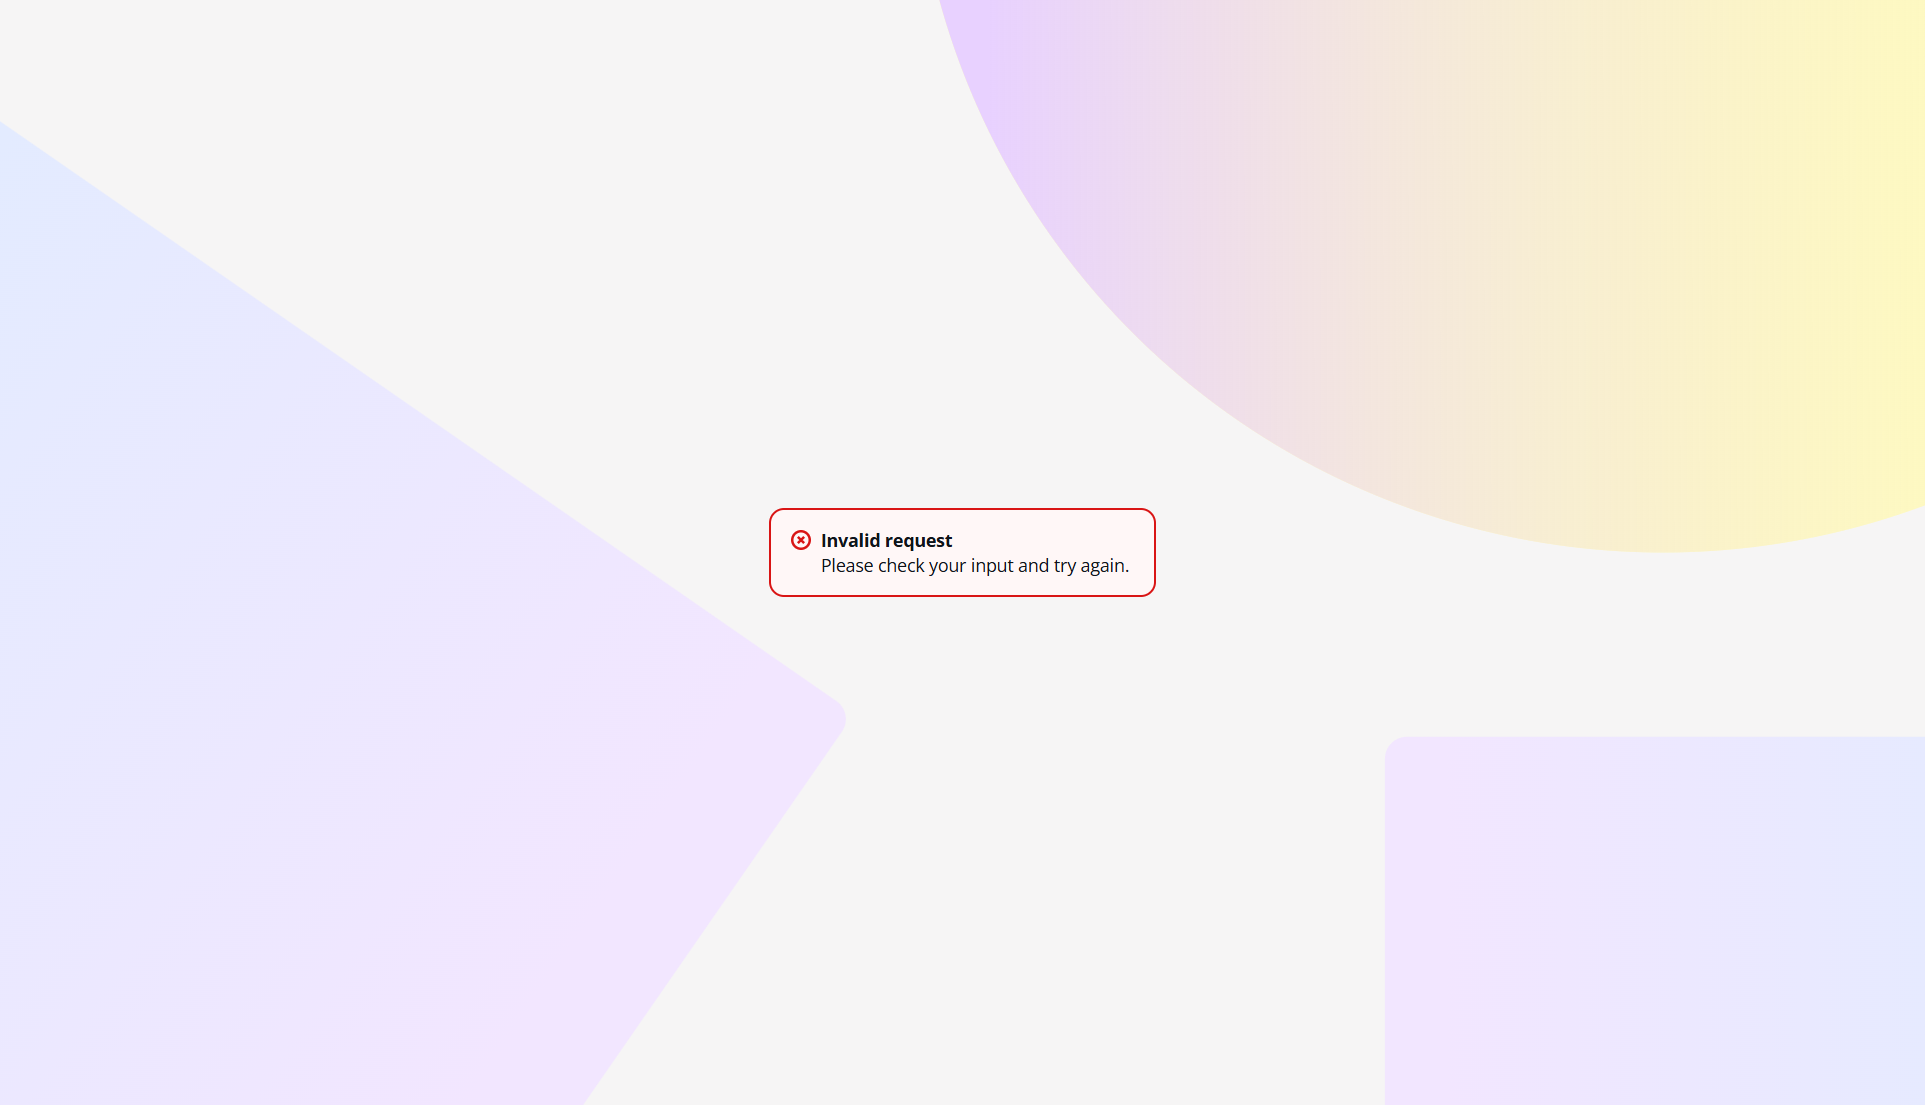
\includegraphics[width=0.88\textwidth]{assets/screenshots/browser/cognito_hosted_ui_login.png}
\caption{Live AWS Cognito Hosted UI Single Sign-On (SSO) Authentication Interface}
\label{fig:cognito_hosted_ui}
\end{figure}
